\section{Auswertung}

Da im Folgenden für alle Rechnungen und Diagramme die Dopplerwinkel gebraucht werden, können zunächst die drei verwendeten Prismenwinkel $\theta = \SI{15}{\degree}$, $\SI{30}{\degree}$ und $\SI{45}{\degree} $ mit Gleichung
\eqref{eqn:alphafinal} umgerechnet werden. Dazu werden die Literaturwerte \cite{skript} aus der Tabelle \ref{tab:lit} entnommen und eingesetzt. Es ergeben sich die Werte
\begin{align*}
    \alpha_{15} &= \SI{80.06}{\degree} \\
    \alpha_{30} &= \SI{70.53}{\degree} \\
    \alpha_{45} &= \SI{54.74}{\degree}.
  \end{align*}

\subsection{Bestimmung der Strömungsgeschwindigkeit}
Die Strömungsgeschwindigkeiten sind je nach Rohrdurchmesser anders, somit lassen sich für alle einzelnen Rohre die Geschwindigkeiten in Abhängigkeit von den drei Dopplerwinkeln bestimmen.
Dazu wird Gleichung \eqref{eqn:deltaf} nach $v$ umgeformt. Es ergibt sich
\begin{equation}
v = \frac{c \increment f}{2 f_{0} \text{cos}(\alpha)}.
\end{equation}
Mit den gemessenen Frequenzverschiebungen $\increment f$, der Grundfrequenz $f_{0} = \SI{2}{\mega\hertz}$ und den unterschiedlichen Winkeln lässt sich nun jede Geschwindigkeit ausrechnen. 
In den folgenden Tabellen \ref{tab:4} bis \ref{tab:6} sind die errechneten Strömungsgeschwindigkeit $v_{ber}$ mit ihren Abhängigkeiten für alle Rohrdurchmesser angegeben.

\begin{table}
    \centering
    \caption{Frequenzverschiebungen und Strömungsgeschwindigkeiten in Abhängigkeit vom Prismenwinkel und der geschalteten Strömungsgeschwindigkeit bei Rohrdurchmesser $\protect d = \SI{7}{\milli\meter}$.}
    \label{tab:4}
    \begin{tabular}{c c c c}
        \toprule
        $v_{\text{gesch}}$ [$\si{{\text{r}}\per\minute}$]  & $\alpha$ [$\si{\degree}$]  & $\increment f$ [$\si{\hertz}$]  &$v_{ber}$ [$\si{\meter\per\second}$] \\
        \midrule
        6000    &   80.06    & 244   & ~ \\ 
        6000    &   70.53    & 366   & ~ \\ 
        6000    &   54.74    & 549   & ~ \\ 
        \midrule
        6500    &   80.06   & 293    & ~ \\ 
        6500    &   70.53   & 415    & ~ \\ 
        6500    &   54.74   & 635    & ~ \\ 
        \midrule
        7000    &   80.06   & 348    & ~ \\ 
        7000    &   70.53   & 500    & ~ \\ 
        7000    &   54.74   & 842    & ~ \\ 
        \midrule
        7500    &   80.06   & 366    & ~ \\ 
        7500    &   70.53   & 623    & ~ \\ 
        7500    &   54.74   & 1001   & ~ \\ 
        \midrule
        8000    &   80.06   & 439    & ~ \\ 
        8000    &   70.53   & 708    & ~ \\ 
        8000    &   54.74   & 1367   & ~ \\ 
        \bottomrule
    \end{tabular}
\end{table}
        
\begin{table}
    \centering
    \caption{Frequenzverschiebungen und Strömungsgeschwindigkeiten in Abhängigkeit vom Prismenwinkel und der geschalteten Strömungsgeschwindigkeit bei Rohrdurchmesser $\protect d = \SI{10}{\milli\meter}$.}
    \label{tab:5}
    \begin{tabular}{c c c c}
        \toprule
        $v_{\text{gesch}}$ [$\si{{\text{r}}\per\minute}$]  & $\alpha$ [$\si{\degree}$]  & $\increment f$ [$\si{\hertz}$] &  $v_{ber}$ [$\si{\meter\per\second}$]\\
        \midrule
        6000    &   80.06    & 434   & ~ \\ 
        6000    &   70.53    & 195   & ~ \\ 
        6000    &   54.74    & 378   & ~ \\ 
        \midrule
        6500    &   80.06   & 159    & ~ \\ 
        6500    &   70.53   & 244    & ~ \\ 
        6500    &   54.74   & 464    & ~ \\ 
        \midrule
        7000    &   80.06   & 171    & ~ \\ 
        7000    &   70.53   & 317    & ~ \\ 
        7000    &   54.74   & 525    & ~ \\ 
        \midrule
        7500    &   80.06   & 195    & ~ \\ 
        7500    &   70.53   & 342    & ~ \\ 
        7500    &   54.74   & 910   & ~ \\ 
        \midrule
        8000    &   80.06   & 220    & ~ \\ 
        8000    &   70.53   & 378    & ~ \\ 
        8000    &   54.74   & 708   & ~ \\ 
        \bottomrule
    \end{tabular}
\end{table}

\begin{table}
    \centering
    \caption{Frequenzverschiebungen und Strömungsgeschwindigkeiten in Abhängigkeit vom Prismenwinkel und der geschalteten Strömungsgeschwindigkeit bei Rohrdurchmesser $\protect d = \SI{16}{\milli\meter}$.}
    \label{tab:6}
    \begin{tabular}{c c c c}
        \toprule
        $v_{\text{gesch}}$ [$\si{{\text{r}}\per\minute}$]  & $\alpha$ [$\si{\degree}$]  & $\increment f$ [$\si{\hertz}$] & $v_{ber}$ [$\si{\meter\per\second}$]\\
        \midrule
        6000    &   80.06    & 61   & ~ \\ 
        6000    &   70.53    & 98   & ~ \\ 
        6000    &   54.74    & 159   & ~ \\ 
        \midrule
        6500    &   80.06   & 85    & ~ \\ 
        6500    &   70.53   & 110    & ~ \\ 
        6500    &   54.74   & 201    & ~ \\ 
        \midrule
        7000    &   80.06   & 98    & ~ \\ 
        7000    &   70.53   & 134    & ~ \\ 
        7000    &   54.74   & 220    & ~ \\ 
        \midrule
        7500    &   80.06   & 110    & ~ \\ 
        7500    &   70.53   & 159    & ~ \\ 
        7500    &   54.74   & 250   & ~ \\ 
        \midrule
        8000    &   80.06   & 110    & ~ \\ 
        8000    &   70.53   & 195    & ~ \\ 
        8000    &   54.74   & 305   & ~ \\ 
        \bottomrule
    \end{tabular}
\end{table}   
                            
Aufgrund der drei Winkel folgen insgesamt drei Geschwindigkeitswerte bei gleichbleibender Zentrifugendrehzahl. Über die Werte lassen sich nun Mittelwerte und ihre Fehler bestimmen.
Der Mittelwert lässt sich durch folgenden Zusammenhang berechnen
\begin{equation}
    \label{eqn:mittel}
\bar{v} = \frac{1}{N} \sum_{i=1}^{N} v_{i}
\end{equation}.
Dabei ist $N$ die Anzahl der Messwerte und $v_{i}$ sind die einzelnen berechneten Geschwindigkeiten.
Der statistische Fehler auf den Mittelwert wird über die Standardabweichung $\sigma$ bestimmt, dafür gilt
\begin{equation}
    \label{eqn:sem}
\increment \bar{v} = \frac{\sigma}{\sqrt{N}} = \sqrt{\frac{1}{N(N-1)} \sum_{i=1}^{N} (v_{i} - \bar{v})^{2}}.
\end{equation}            
                           
                        


\begin{figure}
    \centering
    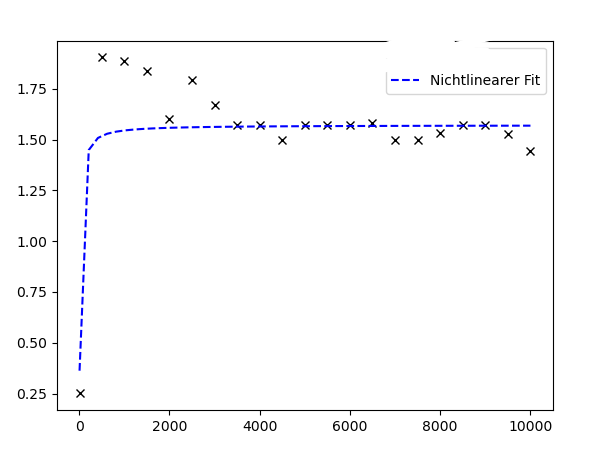
\includegraphics[width=\textwidth]{build/plot1.pdf}
    \caption{Doppler-Prisma als schematischer Querschnitt mit möglichen Winkelkonfigurationen. \cite{skript}} 
    \label{fig:figskizze1}
\end{figure}
\begin{figure}
    \centering
    \includegraphics[width=\textwidth]{build/plot2.pdf}
    \caption{Doppler-Prisma als schematischer Querschnitt mit möglichen Winkelkonfigurationen. \cite{skript}} 
    \label{fig:figskizze1}
\end{figure}
\begin{figure}
    \centering
    \includegraphics[width=\textwidth]{build/plot3.pdf}
    \caption{Doppler-Prisma als schematischer Querschnitt mit möglichen Winkelkonfigurationen. \cite{skript}} 
    \label{fig:figskizze1}
\end{figure}